La planificación del sistema constituye una fase crítica en el desarrollo del
proyecto. Como se mencionó anteriormente en el punto \ref{sec:rt-analysis}, se
cuentan con múltiples tareas que comparten recursos y que se deben ejecutar
con cierta frecuencia para enviar los datos al servidor remoto y detectar los
eventos que se produzcan en el sistema.

El diagrama esquemático que representa al sistema con sus tareas es:

\begin{figure}[H]
  \centering
  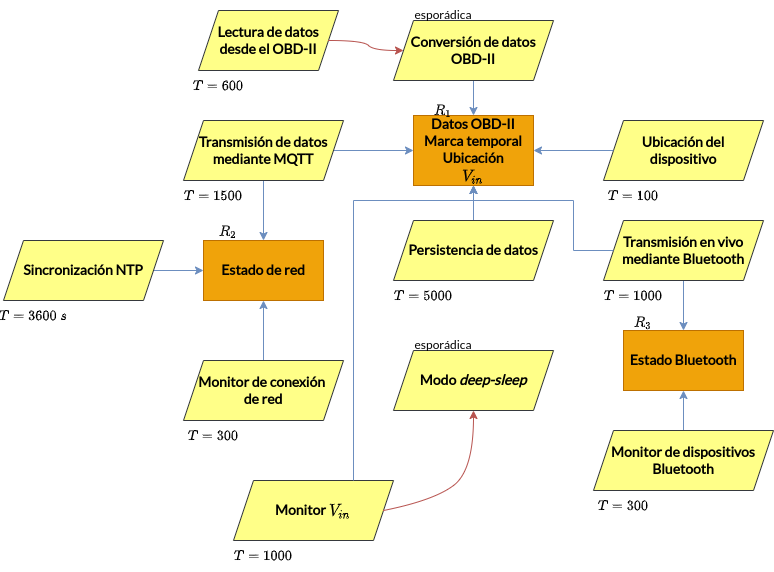
\includegraphics[width=\linewidth]{images/Plannification.png}
  \caption{Diagrama esquemático del sistema con las tareas y objetos protegidos que lo conforman.}
  \label{fig:plannification-diagram}
\end{figure}

En la figura \ref{fig:plannification-diagram} se pueden apreciar las tareas y los
objetos protegidos compartidos por las tareas. En particular, las tareas se representan
por los trapecios amarillos que van acompañados de sus periodos o se indican si son
tareas esporádicas. Los objetos protegidos se representan como rectángulos de color
naranja y se indica, mediante flechas, qué tareas acceden a ellos.

Los datos de las tareas vienen representados en la tabla \ref{tab:rt-table}:

\begin{table}[H]
  \centering
  \begin{tabularx}{\linewidth}{c|X|c|c|c|c|c|c|c}
    $t_i$    & \textbf{Tarea}                         & \textbf{Tipo} & $T_i~\left(ms\right)$ & $D_i~\left(ms\right)$ & $C_i$    & $R_1$      & $R_2$   & $R_3$      \\
    \hline\hline
    $t_{1}$  & Lectura de datos desde \ac{OBD}--II    & $P$           & $600$                 & $400$                 & $C_1$    &            &         &            \\
    $t_{2}$  & Conversión de datos \ac{OBD}--II       & $S$           & $700$                 & $200$                 & $C_2$    & $r^2_1$    &         &            \\
    $t_{3}$  & Sincronización NTP                     & $P$           & $3.6 \cdot 10^6$      & $1000$                & $C_3$    &            & $r^3_2$ &            \\
    $t_{4}$  & Transmisión de datos mediante MQTT     & $P$           & $1500$                & $1500$                & $C_4$    & $r^4_1$    & $r^4_2$ &            \\
    $t_{5}$  & Ubicación del dispositivo              & $P$           & $100$                 & $100$                 & $C_5$    & $r^5_1$    &         &            \\
    $t_{6}$  & Persistencia de datos                  & $P$           & $5000$                & $2000$                & $C_6$    & $r^6_1$    &         &            \\
    $t_{7}$  & Transmisión en vivo mediante Bluetooth & $P$           & $1000$                & $1000$                & $C_7$    & $r^7_1$    &         & $r^7_3$    \\
    $t_{8}$  & Monitor de conexión de red             & $P$           & $300$                 & $300$                 & $C_8$    &            & $r^8_2$ &            \\
    $t_{9}$  & Modo \textit{deep-sleep}               & $S$           & $5000$                & $5000$                & $C_9$    &            &         &            \\
    $t_{10}$ & Monitor $V_{in}$                       & $P$           & $1000$                & $100$                 & $C_{10}$ & $r^{10}_1$ &         &            \\
    $t_{11}$ & Monitor de dispositivos Bluetooth      & $P$           & $300$                 & $300$                 & $C_{11}$ &            &         & $r^{11}_3$ \\
    \hline
  \end{tabularx}
  \caption{Tareas del sistema \ac{VIMS}.}
  \label{tab:rt-table}
\end{table}

Como se puede apreciar en la tabla anterior, las tareas no tienen definido ningún valor
para el uso de CPU ni para el tiempo de acceso a recursos. Estas mediciones se realizan
en laboratorio y suelen llevar un tiempo considerable. Aquí, se sigue el siguiente
modelo para establecer el tiempo de CPU:

\begin{enumerate}
  \item Si una tarea esporádica tiene prioridad \textit{hardware}, su tiempo de CPU
        debe ser muy pequeño.
  \item Si la tarea lee datos de un sensor, el tiempo de cómputo aumenta debido a
        posibles saturaciones del sensor o \textit{delay} en la comunicación.
  \item Para las tareas que leen datos desde el conector \ac{OBD}--II, el tiempo de
        cómputo base aumenta debido a los retardos producidos en la comunicación.
        El puerto \ac{CAN} opera a $1~Mbps$ pero nuestras comunicaciones serán a
        $500~Kbps$, por lo que para los datos que se tienen que recoger en general
        en cada activación (aproximadamente unos $100~bytes$ según los datos de
        las tablas definidas en la sección \ref{sec:maths}) se tiene un tiempo
        de cómputo mínimo de $5$ unidades en lo referente a transmisiones.
  \item Si una tarea trabaja con tipos no primitivos (\textit{arrays}, vectores,
        estructuras, números en coma flotante, \dots) el tiempo de cómputo aumentará.
  \item Si una tarea accede a un recurso protegido, su tiempo de cómputo aumentará
        debido a la lógica de adquirir el \textit{lock} que protege la zona de
        exclusión mutua.
  \item Si una tarea realiza comunicaciones de red, el tiempo de cómputo aumentará
        significativamente debido a los retrasos producidos de dicha comunicación
        y la lógica de enviar datos por la red. Además, para garantizar la
        planificabilidad del sistema, se establece un tiempo máximo de $0.75 \cdot D_i$
        para realizar las comunicaciones de red. En otro caso, serán abortadas.
  \item Si una tarea realiza operaciones de lectura/escritura en disco, su tiempo de
        cómputo aumentará debido a las operaciones de gestión de disco y el \textit{IO Wait}.
\end{enumerate}

Por otra parte, la escritura de datos en los objetos protegidos tendrá un tiempo de
acceso variante según el tipo de dato que se quiera escribir. De esta forma, la
escritura de tipos de datos primitivos se realizarán en un ciclo de instrucción
mientras que la escritura de datos no primitivos (\textit{arrays}, estructuras, etc.)
se realizará en múltiples ciclos de instrucción.

Con esto en mente, se establecen los siguientes $C_i$ y $r^i_j$ para las tareas del sistema
(tabla \ref{tab:ci-rij}):

\begin{table}[H]
  \centering
  \begin{tabular}{|c|c|c|c|c|}
    \hline
    $t_i$    & $C_i$ & $R_1$ & $R_2$ & $R_3$ \\
    \hline
    $t_1$    & $50$  & -     & -     & -     \\
    $t_2$    & $40$  & $15$  & -     & -     \\
    $t_3$    & $30$  & -     & $1$   & -     \\
    $t_4$    & $70$  & $30$  & $1$   & -     \\
    $t_5$    & $20$  & $5$   & -     & -     \\
    $t_6$    & $100$ & $20$  & -     & -     \\
    $t_7$    & $50$  & $20$  & -     & $2$   \\
    $t_8$    & $50$  & -     & $1$   & -     \\
    $t_9$    & $10$  & -     & -     & -     \\
    $t_{10}$ & $15$  & $2$   & -     & -     \\
    $t_{11}$ & $50$  & -     & -     & $2$   \\
    \hline
  \end{tabular}
  \caption{Tiempos de cómputo y acceso a recursos estimados para las tareas del sistema.}
  \label{tab:ci-rij}
\end{table}

Con los datos anteriores ya se puede construir la tabla \ref{tab:rt-table} sustituyendo
los valores simbólicos por sus correspondientes numéricos. Además, se ordenan las tareas
por prioridades basándose en su $D_i$ (\textit{deadline}) ya que se sigue un esquema
\ac{DMS}. El resultado se muestra en la tabla \ref{tab:rt-table-fulfilled}:

\begin{table}[H]
  \centering
  \begin{tabularx}{\linewidth}{c|X|c|c|c|c|c|c|c}
    $t_i$ -- $P_i$   & \textbf{Tarea}                         & \textbf{Tipo} & $T_i~\left(ms\right)$ & $D_i~\left(ms\right)$ & $C_i$ & $R_1$ & $R_2$ & $R_3$ \\
    \hline\hline
    $t_{5}$ -- $11$  & Ubicación del dispositivo              & $P$           & $100$                 & $100$                 & $20$  & $5$   & -     & -     \\
    $t_{10}$ -- $10$ & Monitor $V_{in}$                       & $P$           & $1000$                & $100$                 & $15$  & $2$   & -     & -     \\
    $t_{2}$ -- $9$   & Conversión de datos \ac{OBD}--II       & $S$           & $700$                 & $200$                 & $40$  & $15$  & -     & -     \\
    $t_{8}$ -- $8$   & Monitor de conexión de red             & $P$           & $300$                 & $300$                 & $50$  & -     & $1$   & -     \\
    $t_{11}$ -- $7$  & Monitor de dispositivos Bluetooth      & $P$           & $300$                 & $300$                 & $50$  & -     & -     & $2$   \\
    $t_{1}$ -- $6$   & Lectura de datos desde \ac{OBD}--II    & $P$           & $600$                 & $400$                 & $50$  & -     & -     & -     \\
    $t_{7}$ -- $5$   & Transmisión en vivo mediante Bluetooth & $P$           & $1000$                & $1000$                & $50$  & $20$  & -     & $2$   \\
    $t_{4}$ -- $4$   & Transmisión de datos mediante MQTT     & $P$           & $1500$                & $1500$                & $70$  & $30$  & $1$   & -     \\
    $t_{3}$ -- $3$   & Sincronización NTP                     & $P$           & $3.6 \cdot 10^6$      & $1000$                & $30$  & -     & $1$   & -     \\
    $t_{6}$ -- $2$   & Persistencia de datos                  & $P$           & $5000$                & $2000$                & $100$ & $20$  & -     & -     \\
    $t_{9}$ -- $1$   & Modo \textit{deep-sleep}               & $S$           & $5000$                & $5000$                & $10$  & -     & -     & -     \\
    \hline
  \end{tabularx}
  \caption{Tareas del sistema \ac{VIMS} ordenadas según su prioridad (\ac{DMS}).}
  \label{tab:rt-table-fulfilled}
\end{table}

Sabiendo los datos anteriores, se puede conocer de antemano si el sistema es
planificable o si es necesario realizar el análisis del tiempo de respuesta. Para
ello, se hace uso del ``test basado en el uso de la CPU'' el cual enuncia que
(ecuación \ref{eq:cpu-test}):

\begin{equation}\label{eq:cpu-test}
  U \equiv \sum_{i = 1}^N \left(\frac{C_i}{T_i}\right) \le N \cdot \left(2^{\nicefrac{1}{N}} - 1\right)
\end{equation}

donde se tiene que:

\begin{equation*}
  \left\{
  \begin{aligned}
    U   & : \text{uso de la CPU.}                       \\
    N   & : \text{número de tareas.}                    \\
    C_i & : \text{tiempo de cómputo para la tarea $i$.} \\
    T_i & : \text{periodo para la tarea $i$.}
  \end{aligned}
  \right.
\end{equation*}

Para los datos de entrada dispuestos en la tabla \ref{tab:rt-table-fulfilled} y expandiendo
la ecuación \ref{eq:cpu-test}, se tiene que:

\begin{gather}\label{eq:cpu-test-done}
  \begin{multlined}
    \frac{20}{100} + \frac{15}{1000} + \frac{40}{700} + \frac{50}{300} + \frac{50}{300}%
    + \frac{50}{600} + \frac{50}{1000} + \frac{70}{1500} + \frac{30}{3.6 \cdot 10^6}%
    + \frac{100}{5000} + \frac{10}{5000} \\
    \le 11 \cdot \left(2^{\nicefrac{1}{11}} - 1\right)
  \end{multlined} \\[1ex]
  0.80748 \nleq 0.71545
\end{gather}

Por tanto, al no cumplirse el test, se debe realizar el análisis del tiempo de respuesta
para ver si el sistema es planificable. El proceso es el siguiente:

\begin{enumerate}
  \item Se computa el tiempo máximo de bloqueo de una tarea, según el protocolo \ac{ICPP}.
  \item Se obtiene el \textit{jitter} para las tareas esporádicas presentes en el sistema.
  \item Se realiza el análisis del tiempo de respuesta para el conjunto de tareas teniendo
        en cuenta el valor del \textit{jitter}.
\end{enumerate}

El cómputo del tiempo máximo de bloqueo de una tarea viene determinado por la herencia
de prioridades de cada tarea. Este cómputo viene determinado por la ecuación \ref{eq:block-time}:

\begin{equation}\label{eq:block-time}
  B_i = \max_{k = 1}^k \left(usage\left(k, i\right) \cdot C\left(k\right)\right)
\end{equation}

donde $usage\left(k, i\right)$ determina si una tarea `$i$' usa un recurso `$k$'
y se define como:

\begin{equation*}
  usage\left(k, i\right) = \left\{
  \begin{aligned}
    1 & ,~\text{si $\exists~v,j$ t.q. $v,j$ usan $k$ y se cumple que: } \left(P_v < P_i \land P_j \ge P_i\right) \\
    0 & ,~\text{en otro caso}
  \end{aligned}
  \right.
\end{equation*}

y $C\left(k\right)$ es el \ac{WCET} en la región crítica `$k$'.

De esta forma, para los datos representados en la tabla \ref{tab:rt-table-fulfilled}
(omitiendo aquellas multiplicaciones por $0$ y elementos duplicados), se tiene que:

\begin{equation*}
  \left\{
  \begin{aligned}
    B_{5}  & = \max\left(1 \cdot 5, 1 \cdot 2, 1 \cdot 15, 1 \cdot 20, 1 \cdot 30\right)            & = 30 \\
    B_{10} & = \max\left(1 \cdot 2, 1 \cdot 15, 1 \cdot 20, 1 \cdot 30\right)                       & = 30 \\
    B_{2}  & = \max\left(1 \cdot 15, 1 \cdot 20, 1 \cdot 30\right)                                  & = 30 \\
    B_{8}  & = \max\left(1 \cdot 1, 1 \cdot 5, 1 \cdot 2, 1 \cdot 15, 1 \cdot 20, 1 \cdot 30\right) & = 30 \\
    B_{11} & = \max\left(1 \cdot 2, 1 \cdot 5, 1 \cdot 2, 1 \cdot 15, 1 \cdot 20, 1 \cdot 30\right) & = 30 \\
    B_{1}  & = \max\left(0\right)                                                                   & = 0  \\
    B_{7}  & = \max\left(1 \cdot 5, 1 \cdot 2, 1 \cdot 15, 1 \cdot 20, 1 \cdot 30\right)            & = 30 \\
    B_{4}  & = \max\left(1 \cdot 5, 1 \cdot 2, 1 \cdot 15, 1 \cdot 20\right)                        & = 20 \\
    B_{3}  & = \max\left(0\right)                                                                   & = 0  \\
    B_{6}  & = \max\left(0\right)                                                                   & = 0  \\
    B_{9}  & = \max\left(0\right)                                                                   & = 0
  \end{aligned}
  \right.
\end{equation*}

Con los datos anteriores, se puede completar la tabla que incluye además los tiempos
de bloqueo:

\begin{table}[H]
  \centering
  \begin{tabularx}{\linewidth}{c|X|c|c|c|c|c|c|c|c}
    $t_i$ -- $P_i$   & \textbf{Tarea}                         & \textbf{Tipo} & $T_i~\left(ms\right)$ & $D_i~\left(ms\right)$ & $C_i$ & $R_1$ & $R_2$ & $R_3$ & $B_i$ \\
    \hline\hline
    $t_{5}$ -- $11$  & Ubicación del dispositivo              & $P$           & $100$                 & $100$                 & $20$  & $5$   & -     & -     & $30$  \\
    $t_{10}$ -- $10$ & Monitor $V_{in}$                       & $P$           & $1000$                & $100$                 & $15$  & $2$   & -     & -     & $30$  \\
    $t_{2}$ -- $9$   & Conversión de datos \ac{OBD}--II       & $S$           & $700$                 & $200$                 & $40$  & $15$  & -     & -     & $30$  \\
    $t_{8}$ -- $8$   & Monitor de conexión de red             & $P$           & $300$                 & $300$                 & $50$  & -     & $1$   & -     & $30$  \\
    $t_{11}$ -- $7$  & Monitor de dispositivos Bluetooth      & $P$           & $300$                 & $300$                 & $50$  & -     & -     & $2$   & $30$  \\
    $t_{1}$ -- $6$   & Lectura de datos desde \ac{OBD}--II    & $P$           & $600$                 & $400$                 & $50$  & -     & -     & -     & $0$   \\
    $t_{7}$ -- $5$   & Transmisión en vivo mediante Bluetooth & $P$           & $1000$                & $1000$                & $50$  & $20$  & -     & $2$   & $30$  \\
    $t_{4}$ -- $4$   & Transmisión de datos mediante MQTT     & $P$           & $1500$                & $1500$                & $70$  & $30$  & $1$   & -     & $20$  \\
    $t_{3}$ -- $3$   & Sincronización NTP                     & $P$           & $3.6 \cdot 10^6$      & $1000$                & $30$  & -     & $1$   & -     & $0$   \\
    $t_{6}$ -- $2$   & Persistencia de datos                  & $P$           & $5000$                & $2000$                & $100$ & $20$  & -     & -     & $0$   \\
    $t_{9}$ -- $1$   & Modo \textit{deep-sleep}               & $S$           & $5000$                & $5000$                & $10$  & -     & -     & -     & $0$   \\
    \hline
  \end{tabularx}
  \caption{Tareas del sistema \ac{VIMS} ordenadas según su prioridad (\ac{DMS}).}
  \label{tab:rt-table-block-times}
\end{table}

Con los datos que ya se tienen, se puede realizar un primer análisis del tiempo
de respuesta de las tareas anteriores. Este análisis constituye una condición
suficiente y necesaria sobre el tiempo de respuesta de las tareas y su \textit{deadline}
de manera que si se cumple que, para un sistema:

\begin{equation*}
  R_i \le D_i, \forall i \in t,~\text{donde `$t$' es el conjunto de todas las tareas}
\end{equation*}

entonces el sistema es planificable. La ecuación que modela el análisis del tiempo
de respuesta viene dada por (ecuación \ref{eq:rta}):

\begin{equation}\label{eq:rta}
  R_i^k = C_i + B_i + \sum_{j \in hp\left(i\right)}  \left\lceil \frac{R_i^{k - 1}}{T_j} \right\rceil \cdot C_j + \left\lceil \frac{R_i^{k - 1}}{T_{int}} \right\rceil \cdot C_{int}
\end{equation}

donde se tiene que:

\begin{equation*}
  \left\{\begin{aligned}
    R_i^k            & : \text{tiempo máximo de respuesta de la tarea $i$ en la iteración $k$.} \\
    C_i              & : \text{WCET de la tarea $i$.}                                           \\
    B_i              & : \text{tiempo máximo de bloqueo de la tarea $i$.}                       \\
    hp\left(i\right) & : \text{conjunto de tareas de mayor prioridad que $i$.}                  \\
    T_j              & : \text{periodo de la tarea $j$.}                                        \\
    C_{int}          & : \text{WCET de la tarea de interrupción.}                               \\
    T_{int}          & : \text{periodo de la tarea de interrupción.}
  \end{aligned}\right.
\end{equation*}

Para la primera iteración ($k = 0$) se establece el valor $R_i^{k - 1} = 0$. El análisisd
el tiempo de respuesta se considera finalizado cuando se obtienen dos tiempos de respuesta
consecutivos iguales para una misma tarea:

\begin{equation*}
  R_i = R_i^k \Longleftrightarrow R_i^k = R_i^{k - 1}
\end{equation*}

De esta forma, resolviendo los tiempos de respuesta de la tabla \ref{tab:rt-table-block-times}
y aplicando la ecuación \ref{eq:rta}, se obtiene la tabla \ref{tab:rt-rta} con los
tiempos de respuesta de cada tarea\footnote{El cálculo y obtención de los tiempos
de respuesta de define en el anexo \ref{chap:rta}, con las múltiples iteraciones
con su correspondiente resolución. Se ha omitido del documento principal por su
extensión.}:

\begin{table}[H]
  \centering
  \begin{tabularx}{\linewidth}{c|X|c|c|c|c|c|c|c|c|c}
    $t_i$ -- $P_i$   & \textbf{Tarea}                         & \textbf{Tipo} & $T_i~\left(ms\right)$ & $D_i~\left(ms\right)$ & $C_i$ & $R_1$ & $R_2$ & $R_3$ & $B_i$ & $R_i$  \\
    \hline\hline
    $t_{5}$ -- $11$  & Ubicación del dispositivo              & $P$           & $100$                 & $100$                 & $20$  & $5$   & -     & -     & $30$  & $50$   \\
    $t_{10}$ -- $10$ & Monitor $V_{in}$                       & $P$           & $1000$                & $100$                 & $15$  & $2$   & -     & -     & $30$  & $65$   \\
    $t_{2}$ -- $9$   & Conversión de datos \ac{OBD}--II       & $S$           & $700$                 & $200$                 & $40$  & $15$  & -     & -     & $30$  & $125$  \\
    $t_{8}$ -- $8$   & Monitor de conexión de red             & $P$           & $300$                 & $300$                 & $50$  & -     & $1$   & -     & $30$  & $175$  \\
    $t_{11}$ -- $7$  & Monitor de dispositivos Bluetooth      & $P$           & $300$                 & $300$                 & $50$  & -     & -     & $2$   & $30$  & $225$  \\
    $t_{1}$ -- $6$   & Lectura de datos desde \ac{OBD}--II    & $P$           & $600$                 & $400$                 & $50$  & -     & -     & -     & $0$   & $265$  \\
    $t_{7}$ -- $5$   & Transmisión en vivo mediante Bluetooth & $P$           & $1000$                & $1000$                & $50$  & $20$  & -     & $2$   & $30$  & $485$  \\
    $t_{4}$ -- $4$   & Transmisión de datos mediante MQTT     & $P$           & $1500$                & $1500$                & $70$  & $30$  & $1$   & -     & $20$  & $565$  \\
    $t_{3}$ -- $3$   & Sincronización NTP                     & $P$           & $3.6 \cdot 10^6$      & $1000$                & $30$  & -     & $1$   & -     & $0$   & $575$  \\
    $t_{6}$ -- $2$   & Persistencia de datos                  & $P$           & $5000$                & $2000$                & $100$ & $20$  & -     & -     & $0$   & $1150$ \\
    $t_{9}$ -- $1$   & Modo \textit{deep-sleep}               & $S$           & $5000$                & $5000$                & $10$  & -     & -     & -     & $0$   & $1090$ \\
    \hline
  \end{tabularx}
  \caption{Tareas del sistema \ac{VIMS} ordenadas según su prioridad (\ac{DMS}) y con su tiempo de respuesta.}
  \label{tab:rt-rta}
\end{table}

El siguiente paso a realizar es el cálculo del \textit{jitter}, que aplica únicamente
a las tareas esporádicas. El \textit{jitter} surge cuando una tarea $t_i$ tiene que
activar a otra tarea $t_j$. Como la tarea $t_i$ tiene su propio retardo en la respuesta,
la tarea $t_j$ no se activa tan pronto como se espera sino que va con cierto retraso.
A dicho retraso se le conoce como \textit{jitter}.

El \textit{jitter} se obtiene mediante la siguiente ecuación (ecuación \ref{eq:jitter}):

\begin{equation}\label{eq:jitter}
  J_s = R_p - C_p, \left\{\begin{aligned}
    J_s & : \text{\textit{jitter} de la tarea esporádica $t_s$.} \\
    R_p & : \text{tiempo de respuesta de la tarea $t_p$.}        \\
    C_p & : \text{\ac{WCET} de la tarea $t_p$}
  \end{aligned}\right.
\end{equation}

En el caso del sistema, hay dos tareas esporádicas: $t_2$ y $t_9$, las cuales son
activadas respectivamente por $t_1$ y $t_10$. Por ende, se tendrían los siguientes
valores de \textit{jitter} (ecuación \ref{eq:jitter-values}):

\begin{gather}\label{eq:jitter-values}
  J_2 = R_1 - C_1 = 265 - 50 = 215 \\
  J_9 = R_{10} - C_{10} = 65 - 15 = 50
\end{gather}

De esta forma, actualizando la tabla con los valores, se tiene (tabla \ref{tab:rt-table-jitter}):

\begin{table}[H]
  \centering
  \begin{tabularx}{\linewidth}{c|X|c|c|c|c|c|c|c|c|c|c}
    $t_i$ -- $P_i$   & \textbf{Tarea}                         & \textbf{Tipo} & $T_i~\left(ms\right)$ & $D_i~\left(ms\right)$ & $C_i$ & $R_1$ & $R_2$ & $R_3$ & $B_i$ & $R_i$  & $J_i$ \\
    \hline\hline
    $t_{5}$ -- $11$  & Ubicación del dispositivo              & $P$           & $100$                 & $100$                 & $20$  & $5$   & -     & -     & $30$  & $50$   & -     \\
    $t_{10}$ -- $10$ & Monitor $V_{in}$                       & $P$           & $1000$                & $100$                 & $15$  & $2$   & -     & -     & $30$  & $65$   & -     \\
    $t_{2}$ -- $9$   & Conversión de datos \ac{OBD}--II       & $S$           & $700$                 & $200$                 & $40$  & $15$  & -     & -     & $30$  & $125$  & $215$ \\
    $t_{8}$ -- $8$   & Monitor de conexión de red             & $P$           & $300$                 & $300$                 & $50$  & -     & $1$   & -     & $30$  & $175$  & -     \\
    $t_{11}$ -- $7$  & Monitor de dispositivos Bluetooth      & $P$           & $300$                 & $300$                 & $50$  & -     & -     & $2$   & $30$  & $225$  & -     \\
    $t_{1}$ -- $6$   & Lectura de datos desde \ac{OBD}--II    & $P$           & $600$                 & $400$                 & $50$  & -     & -     & -     & $0$   & $265$  & -     \\
    $t_{7}$ -- $5$   & Transmisión en vivo mediante Bluetooth & $P$           & $1000$                & $1000$                & $50$  & $20$  & -     & $2$   & $30$  & $485$  & -     \\
    $t_{4}$ -- $4$   & Transmisión de datos mediante MQTT     & $P$           & $1500$                & $1500$                & $70$  & $30$  & $1$   & -     & $20$  & $565$  & -     \\
    $t_{3}$ -- $3$   & NTP                                    & $P$           & $3.6 \cdot 10^6$      & $1000$                & $30$  & -     & $1$   & -     & $0$   & $575$  & -     \\
    $t_{6}$ -- $2$   & Persistencia de datos                  & $P$           & $5000$                & $2000$                & $100$ & $20$  & -     & -     & $0$   & $1150$ & -     \\
    $t_{9}$ -- $1$   & Modo \textit{deep-sleep}               & $S$           & $5000$                & $5000$                & $10$  & -     & -     & -     & $0$   & $1090$ & $50$  \\
    \hline
  \end{tabularx}
  \caption{Tareas del sistema \ac{VIMS} ordenadas según su prioridad (\ac{DMS}) con el valor del \textit{jitter} actualizado.}
  \label{tab:rt-table-jitter}
\end{table}

A continuación, se debe repetir el análisis de tiempo de respuesta teniendo en
consideración los valores de los \textit{jitter}. Para ello, se usa la ecuación
\ref{eq:rta-jitter} que se parece a la fórmula \ref{eq:rta} con ciertos
matices:

\begin{equation}\label{eq:rta-jitter}
  R_i^k = C_i + B_i + \sum_{j \in hp\left(i\right)} \left\lceil\frac{R_i^{k - 1} + J_j}{T_j}\right\rceil\cdot C_j + \left\lceil\frac{R_i^{k - 1} + J_{int}}{T_{int}}\right\rceil\cdot C_{int}
\end{equation}

De esta forma, quedarían los siguientes tiempos de respuesta actualizados que se muestran
en la tabla \ref{tab:rt-table-rta-jitter}\footnote{El cálculo de los nuevos tiempos
de respuesta se encuentra en el anexo \ref{sec:rta-jitter} debido a su extensión. Allí
se pueden encontrar todas las ecuaciones, su desglose y resolución paso a paso}:

\begin{table}[H]
  \centering
  \begin{tabularx}{\linewidth}{c|X|c|c|c|c|c|c|c|c|c|c}
    $t_i$ -- $P_i$   & \textbf{Tarea}                         & \textbf{Tipo} & $T_i~\left(ms\right)$ & $D_i~\left(ms\right)$ & $C_i$ & $R_1$ & $R_2$ & $R_3$ & $B_i$ & $R_i$  & $J_i$ \\
    \hline\hline
    $t_{5}$ -- $11$  & Ubicación del dispositivo              & $P$           & $100$                 & $100$                 & $20$  & $5$   & -     & -     & $30$  & $50$   & -     \\
    $t_{10}$ -- $10$ & Monitor $V_{in}$                       & $P$           & $1000$                & $100$                 & $15$  & $2$   & -     & -     & $30$  & $65$   & -     \\
    $t_{2}$ -- $9$   & Conversión de datos \ac{OBD}--II       & $S$           & $700$                 & $200$                 & $40$  & $15$  & -     & -     & $30$  & $125$  & $215$ \\
    $t_{8}$ -- $8$   & Monitor de conexión de red             & $P$           & $300$                 & $300$                 & $50$  & -     & $1$   & -     & $30$  & $175$  & -     \\
    $t_{11}$ -- $7$  & Monitor de dispositivos Bluetooth      & $P$           & $300$                 & $300$                 & $50$  & -     & -     & $2$   & $30$  & $225$  & -     \\
    $t_{1}$ -- $6$   & Lectura de datos desde \ac{OBD}--II    & $P$           & $600$                 & $400$                 & $50$  & -     & -     & -     & $0$   & $265$  & -     \\
    $t_{7}$ -- $5$   & Transmisión en vivo mediante Bluetooth & $P$           & $1000$                & $1000$                & $50$  & $20$  & -     & $2$   & $30$  & $485$  & -     \\
    $t_{4}$ -- $4$   & Transmisión de datos mediante MQTT     & $P$           & $1500$                & $1500$                & $70$  & $30$  & $1$   & -     & $20$  & $795$  & -     \\
    $t_{3}$ -- $3$   & NTP                                    & $P$           & $3.6 \cdot 10^6$      & $1000$                & $30$  & -     & $1$   & -     & $0$   & $825$  & -     \\
    $t_{6}$ -- $2$   & Persistencia de datos                  & $P$           & $5000$                & $2000$                & $100$ & $20$  & -     & -     & $0$   & $1150$ & -     \\
    $t_{9}$ -- $1$   & Modo \textit{deep-sleep}               & $S$           & $5000$                & $5000$                & $10$  & -     & -     & -     & $0$   & $1090$ & $50$  \\
    \hline
  \end{tabularx}
  \caption{Tareas del sistema \ac{VIMS} ordenadas según su prioridad (\ac{DMS}) con el tiempo de respuesta actualizado según el \textit{jitter}.}
  \label{tab:rt-table-rta-jitter}
\end{table}

Con esto, la planificación del sistema se da por completada y se concluye que el sistema
es planificable.
